\documentclass[../../memoria.tex]{subfiles}

\begin{document}

\paragraph{}
Sobre el \textit{MVP} propuesto para la solución, se han realizados varias pruebas.
\paragraph{}
Estas pruebas se han realizado desde un ordenador portátil con las siguientes características:

\begin{figure}[H]
    \centering
    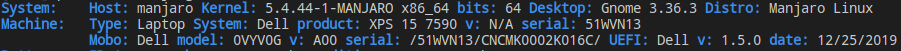
\includegraphics[width=1\columnwidth]{pc-caracteristicas.png}
    \caption{Características del PC desde el cual se han ejecutado las pruebas}
    \label{fig:pcCaracteristicas}
\end{figure}

\paragraph{}
La versión de Grafana \cite{grafana} utilizada en una de las pruebas es la 7.0.2.
\paragraph{}
A continuación, se detallan todas estas pruebas junto con sus resultados. Asimismo, se explicará una prueba de concepto de una hipotética situación a la que se podría enfrentar el sistema.

\end{document}
